\documentclass[english]{tktltiki2}

% --- General packages ---

\usepackage[utf8]{inputenc}
\usepackage[T1]{fontenc}
\usepackage{lmodern}
\usepackage{microtype}
%\usepackage[table,xcdraw]{xcolor}    % loads also »colortbl«
\usepackage{listings}
\usepackage{tabularx}
%\usepackage{minted}
%\usepackage{tcolorbox}
%\usepackage{etoolbox}
%\BeforeBeginEnvironment{minted}{\begin{tcolorbox}}%
%\AfterEndEnvironment{minted}{\end{tcolorbox}}%

\usepackage{amsfonts,amsmath,amssymb,amsthm,booktabs,enumitem,graphicx}
\usepackage{tocloft}
%\usepackage{relsize}
\usepackage[pdftex,hidelinks]{hyperref}
\usepackage[title]{appendix}
%\usepackage{tabularx}
%\usepackage[table]{xcolor}    % loads also »colortbl«
%\usepackage{float}

%\listfiles

\linespread{1.3}

\setlength{\intextsep}{18pt plus 2.0pt minus 2.0pt}

\lstset{%
  language=[LaTeX]TeX,
  basicstyle=\ttfamily,
  breaklines=true,
  columns=fullflexible,
}

%\setlength{\arrayrulewidth}{0.6pt}

% Automatically set the PDF metadata fields
\makeatletter
\AtBeginDocument{\hypersetup{pdftitle = {\@title}, pdfauthor = {\@author}}}
\makeatother

% --- Language-related settings ---
%
% these should be modified according to your language

% babelbib for non-english bibliography using bibtex
\usepackage[fixlanguage]{babelbib}
\selectbiblanguage{english}

% add bibliography to the table of contents
\usepackage[nottoc]{tocbibind}
% tocbibind renames the bibliography, use the following to change it back

\declarebtxcommands{english}{%
    \def\btxurldatecomment#1{ [#1]}%
}

% --- tktltiki2 options ---
%
% The following commands define the information used to generate title and
% abstract pages. The following entries should be always specified:

\title{Mining a Bird Observatory Dataset}
\author{Mikko Koho}
\date{\today}
\level{Technical report}

\abstract{
}

\keywords{}
%\classification{
%\textbf{} \\
%\textit{} \\
%\\
%}
% classification according to ACM Computing Classification System (http://www.acm.org/about/class/)
                  % This is probably mostly relevant for computer scientists

% If the automatic page number counting is not working as desired in your case,
% uncomment the following to manually set the number of pages displayed in the abstract page:
%



\begin{document}
    
% --- Front matter ---

\frontmatter      % roman page numbering for front matter

\maketitle        % title page

\makeabstract     % abstract page

\tableofcontents  % table of contents

% --- Main matter ---

\mainmatter       % clear page, start arabic page numbering


%%%%%%%%%%%%%%%%%%%
\section{Introduction}
%%%%%%%%%%%%%%%%%%%

This technical report examines the use of data mining techniques~\cite{tan2006introduction} to find interesting patterns from a bird observatory dataset.



%%%%%%%%%%%%%%%%%%%
\section{Dataset}
%%%%%%%%%%%%%%%%%%%

Halias bird observatory is located at the southernmost tip of Finland in Hanko, Finland. Halias has been gathering bird observation data from 1979 onward and it has been used intensively in research~\cite{HangonJulkaisut}. However data mining or machine learning methods have been never applied to it, so these methods could perhaps uncover some interesting patterns in the data.

Data gathering at the bird observatory is highly standardized and main focus is on counting the daily migration of each bird species. The data unfortunately is not publicly available, but is available for research projects at request.

The data in digital form consists of two Excel files, containing half a million rows of distinct daily counts per species for local and migrating birds from 1979 to 2009.

However, in this case study we will be using a linked data publication made from the original dataset. The dataset has been transformed~\cite{koho-hyvonen-orni-2014, koho2015gradu} to RDF data model and linked with weather data from nearby weather station in Hanko, Russarö and a bird taxon ontology. %~\cite{tuominen-et-al-avio-2013}.
The linked dataset is structured using the RDF Data Cube Vocabulary~\cite{w3crdfdatacube}, containing distinct data cubes for both daily bird observations and daily weather observations. An example of the data in this format is given in figure \ref{fig: havaintograafi}.

\begin{figure}[htb]
\centering
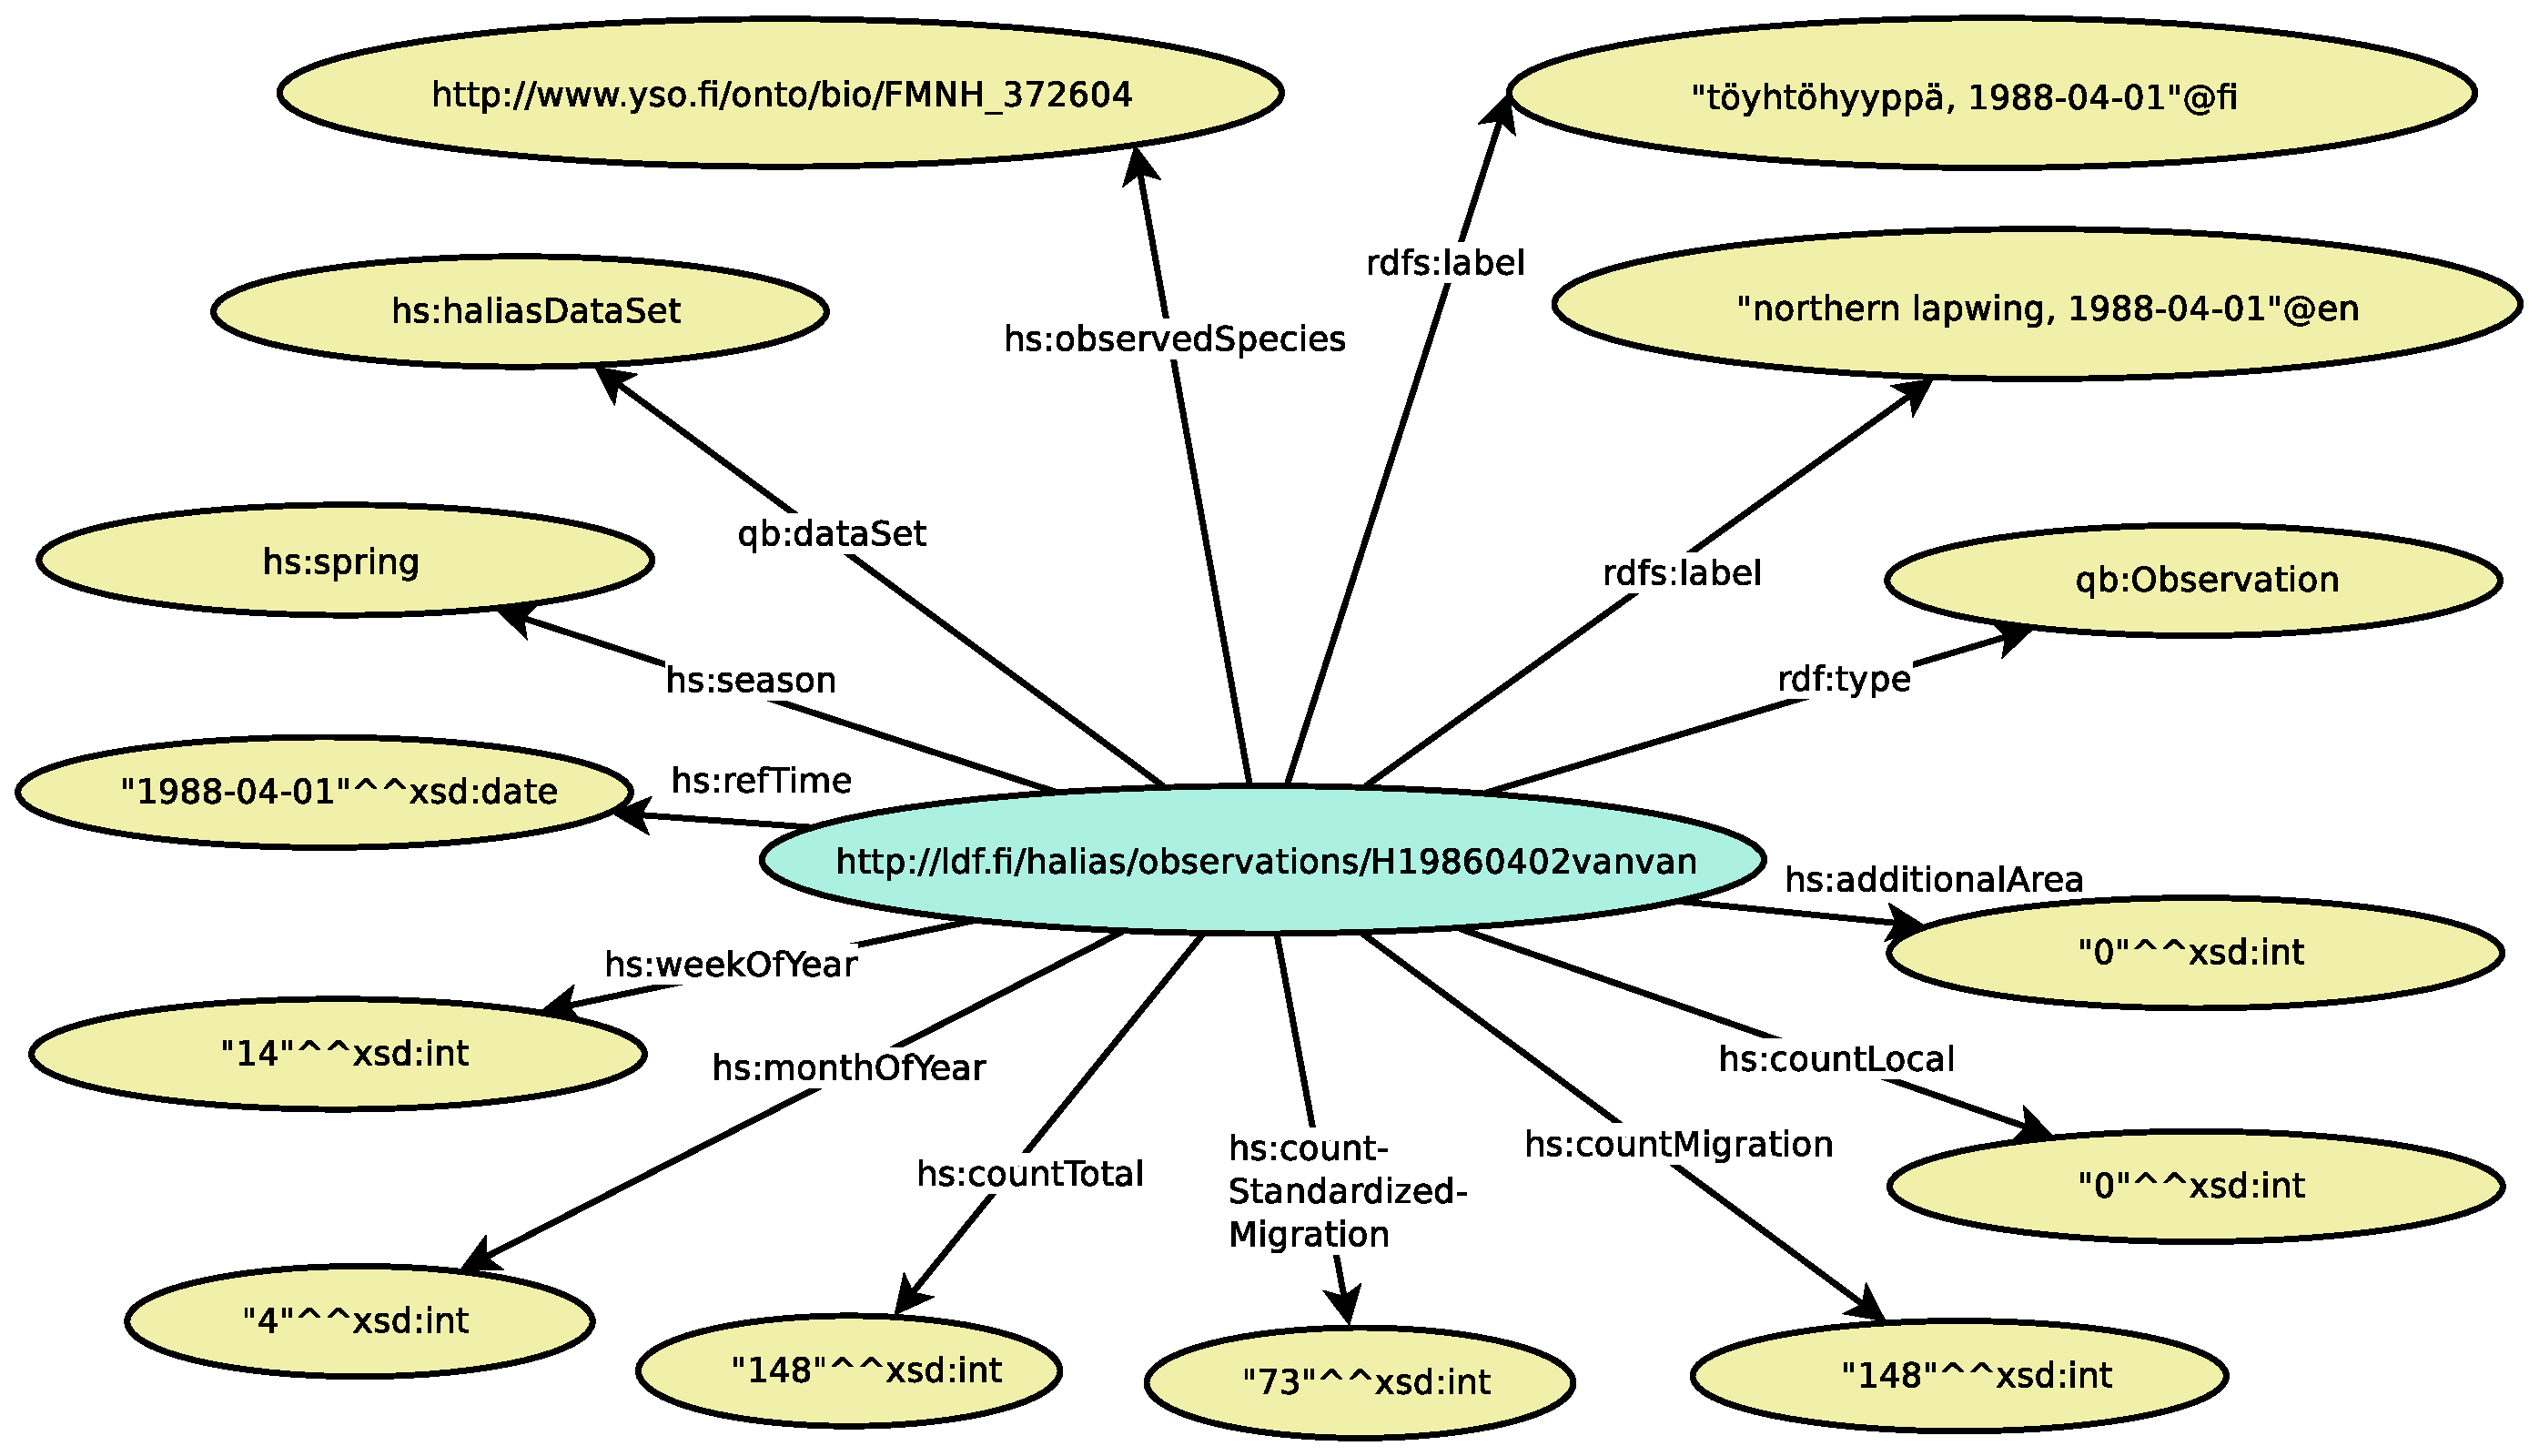
\includegraphics[clip=true, width=\textwidth]{havaintograafi}
\caption{Daily observation data of one species from one day in RDF format~\cite{koho2015gradu}.}
\label{fig: havaintograafi}
\end{figure}



%%%%%%%%%%%%%%%%%%%
\section{Methodology}
%%%%%%%%%%%%%%%%%%%

For association analysis we take a subset of the values in the data cubes and transform these to market basket transactions or sequence database. In this transformation it is easy to combine bird observations, weather observations and information from the used ontologies.

The dataset is very large for many association analysis tasks, and therefore it may be neccessary to aggregate some variables.

For simplicity, we first try to find interesting patterns using just the bird observations. We will do frequent pattern mining to find the most frequently observed species and species combinations, without using the daily counts. We could also use the observed counts and generate quantitative association rules, which might reveal some interesting patterns, but is probably very slow to calculate.

Next, we will try sequential pattern mining, using the timestamps already present in the data. This would probably reveal something interesting, but is again very slow to calculate.

The analysis is done using Python 2.7 and Orange Data Mining Toolbox~\cite{Orange}.


%%%%%%%%%%%%%%%%%%%
\section{Analysis results}
%%%%%%%%%%%%%%%%%%%

\subsection{Frequent itemsets}
%%%%%%%%%%%%%%%%%%%

Analysing daily observed species as market basket transactions, we can see what are the most commonly observed species.
For support $0.5$, the largest frequent itemset consists of the following species. Finnish names are used here for clarity.

\begin{itemize}
\item[] telkkä, sinisorsa, sinitiainen, isokoskelo, viherpeippo, varis, kalalokki, harmaalokki, merilokki, talitiainen
\end{itemize}

This is the largest combination of species that is observed in half of the observation days. These species are very common and observable almost all year round.


\subsection{Rule generation}
%%%%%%%%%%%%%%%%%%%

This dataset was too large for Orange Data Mining Toolbox...

%%%%%%%%%%%%%%%%%%%
\section{Conclusions}
%%%%%%%%%%%%%%%%%%%



%%%%%%%%%%%%%%%%%%%
\section{Discussion}
%%%%%%%%%%%%%%%%%%%



\pagebreak

% --- References ---
%
% bibtex is used to generate the bibliography. The babplain style
% will generate numeric references (e.g. [1]) appropriate for theoretical
% computer science. If you need alphanumeric references (e.g [Tur90]), use
%
% \bibliographystyle{babalpha-lf}
%
% instead.

\bibliographystyle{babalpha-lf}
\bibliography{references-en}

\lastpage

\end{document}
